
\documentclass[12pt,a4paper]{article} % Use A4 paper with a 12pt font size - different paper sizes will require manual recalculation of page margins and border positions

% Generated with LaTeXDraw 2.0.8
% Mon Jun 17 19:00:40 EDT 2013
\usepackage[usenames,dvipsnames]{pstricks}
\usepackage{epsfig}
\usepackage{pst-grad} % For gradients
\usepackage{pst-plot} % For axes
<<<<<<< HEAD
\usepackage{marginnote} % Required for margin notes
\usepackage{wallpaper} % Required to set each page to have a background
\usepackage{lastpage} % Required to print the total number of pages
\usepackage[left=1.3cm,right=4.6cm,top=1.8cm,bottom=4.0cm,marginparwidth=3.4cm]{geometry} % Adjust page margins
=======
%\usepackage{marginnote} % Required for margin notes
%\usepackage{wallpaper} % Required to set each page to have a background
%\usepackage{lastpage} % Required to print the total number of pages
%\usepackage[left=1.3cm,right=4.6cm,top=1.8cm,bottom=4.0cm,marginparwidth=3.4cm]{geometry} % Adjust page margins
>>>>>>> b8525e412146e0fcfdf863db5f2485f1d3879535
\usepackage{amsmath} % Required for equation customization
\usepackage{amssymb} % Required to include mathematical symbols
\usepackage{xcolor} % Required to specify colors by name
\usepackage{amsthm}
\usepackage{float}


\setlength{\parindent}{0cm} % Remove paragraph indentation
\newcommand{\tab}{\hspace*{2em}} % Defines a new command for some horizontal space


<<<<<<< HEAD
\title{Calculus and Linear Algebra Workshop Notes and Problems - Basics of Derivatives and Differentiation}
=======
\title{Calculus and Linear Algebra Workshop Notes and Problems - Basics of Integration}
>>>>>>> b8525e412146e0fcfdf863db5f2485f1d3879535
%----------------------------------------------------------------------------------------

\newtheorem{defn}{Definition}
\newtheorem{example}{Example}
\newtheorem{prop}{Proposition}
\newtheorem{exer}{Exercises}
\newtheorem{thm}{Therorem}
\begin{document}
\maketitle
<<<<<<< HEAD
\section{Integration}
Like the derivative, the definite integral is defined as a limit.
\begin{defn}
Let $f$ be a function defined on the interval $[a,b]$. We define the definite integral of $f$ on $[a,b]$ as:
$$\int_a^bf(x)dx	=	\lim_{\max(\Delta x_k)\rightarrow 0}\sum_{k=1}^nf(x_k^*)\Delta x_k$$
where $a=x_1\leq x_2\leq ... \leq x_n=b$ is a partition of the interval $[a,b]$, $\Delta_k = x_{k+1}-x_k$ for $k=1,...,n-1$ and $x_k\leq x_k^*\leq x_{k+1}$. 
\end{defn}
Each term in the sum above is the area of a rectangle, with height $f(x_k^*)$ and width $x_{k+1}-x_k$. In the limit, we make the width of the rectangles approach zero. The quantity we calculate is the area under the curve of the function $f(x)$ on the interval $[a,b]$.
\subsection{Computing Definite Integrals}

=======
\section{Definition of Definite Integral}
Like the derivative, the definite integral is defined as a limit.
\begin{defn}
Let $f$ be a function defined on the interval $[a, b]$. We define the definite
integral of $f$ on $[a, b]$ as:
$$\int_a^b f(x)dx = \lim_{\max(\Delta_x)\rightarrow 0}\sum_{k=1}^n f (x^∗_k )\Delta x_k$$
where $a = x_1 \leq x_2 \leq ... \leq x_n = b$ is a partition of the interval $[a, b]$ and $\Delta x_k = x_{k+1} − x_k$
for $k = 1, ..., n − 1$ and $x_k \leq x^∗_k \leq x_{k+1}$.
\end{defn}
Each term in the sum above is the area of a rectangle, with height $f (x^∗_k)$ and width
$x_{k+1} − x_k$. In the limit, we make the width of the rectangles approach zero. The
quantity we calculate is the area under the curve of the function $f(x)$ on the interval
$[a, b]$.\\
Most calculus courses first define particular "Riemann Sums". The following figure illustrates 3 different sums - the left hand sum, the right hand sum and the mid-point. These are just different choices for $x^*_k$. \\\\

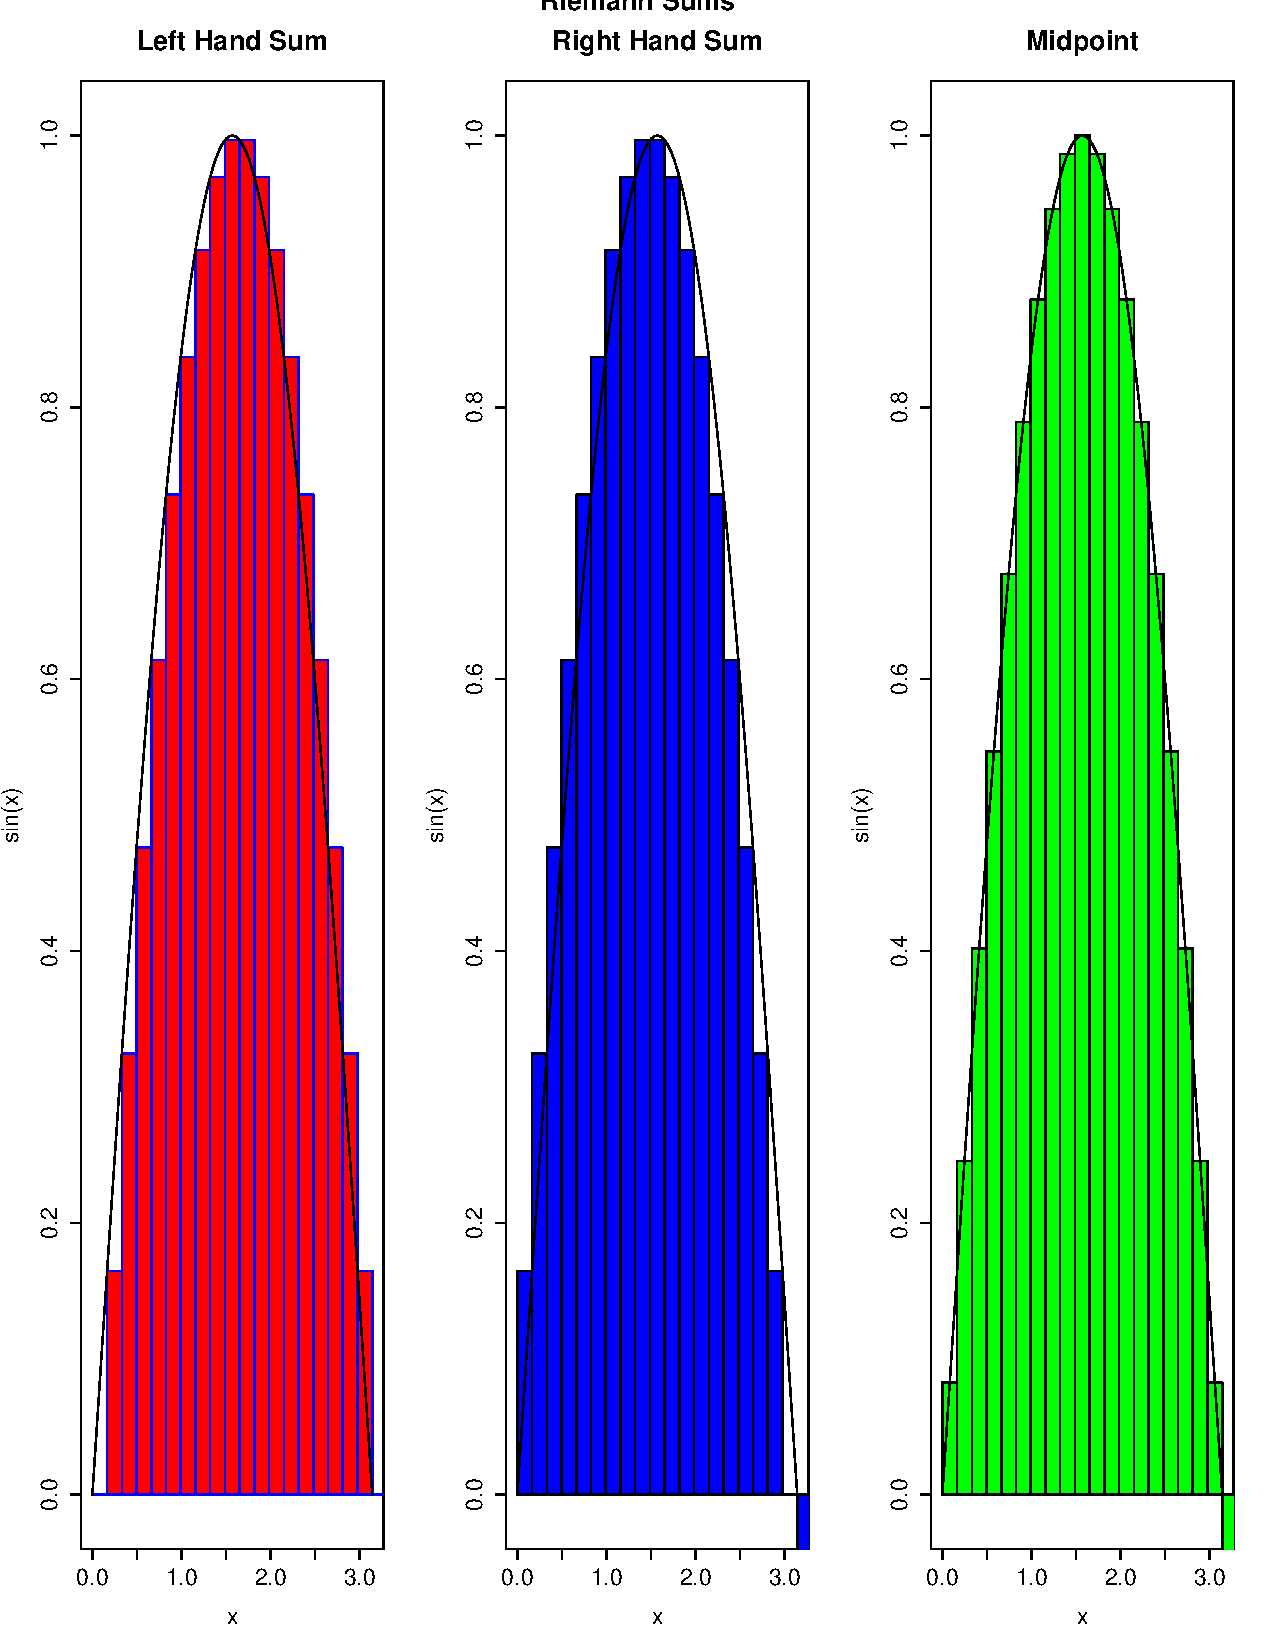
\includegraphics[width = 6in,height=3in]{RSums.pdf}

Clearly, in the limit that the intervals shrink to zero, it doesn't matter which $x^*_k$ we choose:\\\\

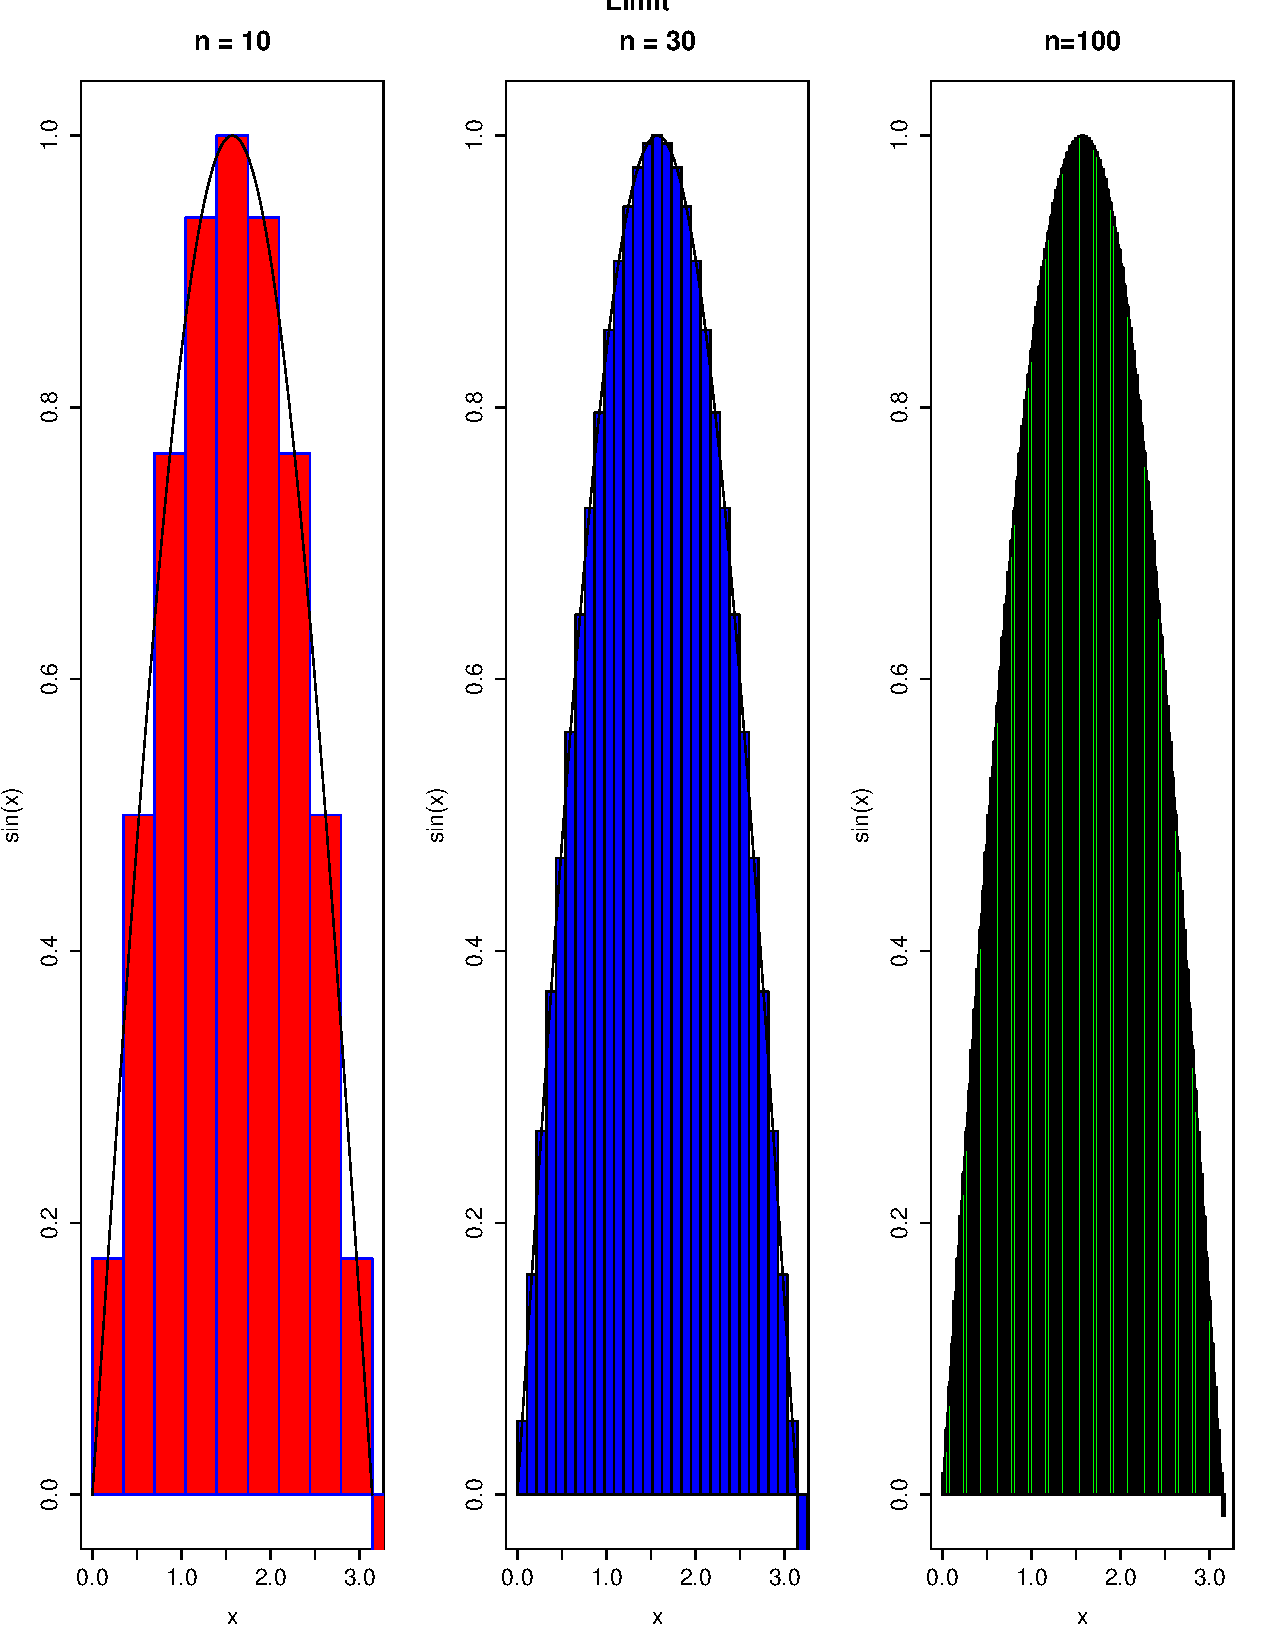
\includegraphics[width = 6in, height=3in]{IntLimit.pdf}
\section{Properties of Integrals}
The following are useful properties of the integral:
\begin{itemize}
\item Linearity:
$$\int cf(x)dx = c\int f(x) dx \textrm{ and } \int(f(x)+g(x))dx = \int f(x)dx + \int g(x) dx$$
\item $$\int_a^b f(x) dx = -\int_b^a f(x) dx$$
\item $$ \int_a^a f(x) dx = 0$$
\item For any $c$ such that $a\leq c\leq b$
$$\int_a^bf(x)dx = \int_a^c f(x) dx + \int_c^b f(x) dx$$ 
\end{itemize}
\section{Computing Integrals and the Fundamental Theorem of Calculus}
Now, we do not want to have to compute the limit of areas of rectangles and fortunately, we don't have to. The fundamental theorem tells us that:
$$\int_a^b f(x) dx = F(b) - F(a)$$
where $F$ is an \emph{anti-derivative} of $f$, i.e.
$$F'(x) = f(x)$$
\subsection{Common Integration Techniques}
\subsubsection{Power Rule}
\begin{thm}
The indefinite integral of $x^n$, for $n\neq 1$ is
$$\int x^n dx = \frac{x^{n+1}}{n+1} + C\textrm{ for } n\neq 1$$ 
\end{thm} 
Note that $n$ \emph{need not be an integer}. 
\subsubsection{Indefinite Integrals of Commonly Used Functions}
Note: indefinite integrals (anti-derivatives) are not unique. Because the derivative of a constant is zero, we can add any constant to an indefinite integral and it is still correct. In the following, we will ignore this and simply write the anti-derivative where the constant $C=0$. 
\begin{itemize}
\item $$\int \frac1{x} dx = \log(x)$$
\item $$\int e^x dx= e^x$$
\item $$\int \sin(x) dx = -\cos(x)$$
\item $$\int \cos(x) = \sin(x)$$
\end{itemize}
\subsubsection{Substitution}
What do we do when we do not automatically see the derivative of a function - but we see that there may be a composite function we are dealing with? In other words, our integrand looks like something of the form:
$$f'(g(x))g'(x)$$
In other words, it looks like the result of differentiation using the chain rule. Well, we try to find $g(x)$ and substitute into the integral. The trick is that we must not only substitute our integrand - we also need to substitute the differential $dx$. This is best seen by example:
\begin{example}
Compute the indefinite integral:
$$\int x e^{-x^2} dx$$
First, we let $u=-x^2$. If we make that substitution, we have to substitute:
$$du = -2x dx$$ 
Now, it looks like our integral \emph{almost} has the form $e^{u} du$ - BUT - we are missing a factor of $-2$. That is easy to deal with - we just multiply by $-2$ inside the integral, and divide by $-2$ outside: 
Therefore:
$$\int x e^{-x^2} dx = -\frac12 \int -2x e^{-x^2}dx = -\frac12\int e^u du = -e^u + C$$
Now, we just back-substitute:
$$\int x e^{-x^2} dx = -\frac12e^{-x^2} + C$$
\end{example}
Here are a bunch for you to try:
\begin{itemize}
\item $$\int \frac{x}{x^2+1}$$
\item $$\int \cos(\cos(x))\sin(x)dx$$
\item $$x^2 e^{-4x^3}dx$$
\end{itemize}
\subsubsection{Integration by Parts}
Integration by parts is kind of the Hail Mary play of integration. We don't know what else to do, and it looks like splitting the integrand into a product might work (integration by parts is sometimes called the 'inverse product rule). The formula is as follows:
$$\int u dv = uv - \int v du$$
Let's do an example that we saw in class:
$$\int x e^{-x} dx$$
Let $u = x$ and $dv = e^{-x} dx$. Then $du = dx$ (yay!) and $v=-e^{-x}$, so
$$\int x e^{-x} dx = -xe^{-x} + \int e^{-x} dx$$
$$= -xe^{-x} - e^{-x} + C$$
Your turn!
\begin{itemize}
\item $$\int\log(x) dx$$
\item $$\int \sqrt{x} \log(x) dx$$
\item $$\int x \sin(x) dx$$
\end{itemize}
>>>>>>> b8525e412146e0fcfdf863db5f2485f1d3879535
\end{document}